
\documentclass[conference,a4paper]{IEEEtran}

\usepackage[utf8]{inputenc}

\usepackage[pdftex]{graphicx}
\graphicspath{{./img/}{./jpeg/}}
\DeclareGraphicsExtensions{.pdf,.jpeg,.png}

\usepackage[cmex10]{amsmath}

\DeclareRobustCommand*{\IEEEauthorrefmark}[1]{\raisebox{0pt}[0pt][0pt]{\textsuperscript{\footnotesize #1}}}

\begin{document}

\title{Asynchronous Multi-Ported Memory Controllers for FPGAs}

\author{
	\IEEEauthorblockN{
		M. Sánchez de León\IEEEauthorrefmark{1},
		H. Liu\IEEEauthorrefmark{2}
	}
	\IEEEauthorblockA{\IEEEauthorrefmark{1}
	Supélec University, France, miguel.sanchezdeleonpeque@supelec.fr}
	\IEEEauthorblockA{\IEEEauthorrefmark{2}
	Supélec University, France, hongjie.liu@supelec.fr}
}

\maketitle


\begin{abstract}
Multi-ported memories are challenging to implement in FPGAs since the provided block RAMs typically have only two ports. We propose a new approach and introduce an asynchronous memory controller in order to minimize the delay between requests and responses.
\end{abstract}

{\smallskip \keywords FPGA, memory, multi-port, parallel, asynchronous.}

\IEEEpeerreviewmaketitle

\vspace{7pt}
\section{Introduction}

Nowadays, heterogeneous architectures are becoming more and more popular. The fact that some tasks can be accelerated carrying out many calculations simultaneously in different processing units has lead to the development of massively parallel processors, as the modern and affordable General Purpose Graphics Processing Units (GPGPUs).

These architectures have also complex memory configurations, stepping away from the classical Von-Newmann model. Implementing multiple processing units with access to an external global memory in a FPGA is possible with most current development boards, but the problem comes when trying to implement on-chip multiported shared memories with high throughput and capacity. That is the problem we are addressing in this paper.

There are several classical ways to implement multiported memories in a FPGA:

\begin{itemize}
  \item Pure Adaptative Logic Module (ALM) implementations, using their generic reconfigurable logic. Although this memories have virtually no constraints on capacity, configuration and number of ports, they pay a large area and speed penalty.
  \item Replication is a kind of approach which increases the number of read ports by maintaining a copy of the memory for each additional read port. The disadvantange is that this technique is limited to only one write port, which must be routed to every Block RAM (BRAM).
  \item Banking allows each additional bank to support an additional read and write port by dividing memory locations. However, a pure banked design does not truly support sharing accross ports, which means each read or write port is limited to only one memory division.
  \item With multi-pumping methods, all the memory design is clocked at a multiple of the external clock, providing the illusion of a multiple of the number of ports. The drawback of a multi-pumped design is that each increase in the number of ports dramatically reduces the maximum external operating frequency of the memory.
\end{itemize}

A more efficient approach was developped in 2010 \cite{LaForest}, and later improved in 2012 \cite{LaForestXOR}: Live Value Table (LVT) memories (Fig. \ref{lvt}).

\begin{figure}[h]
\centering
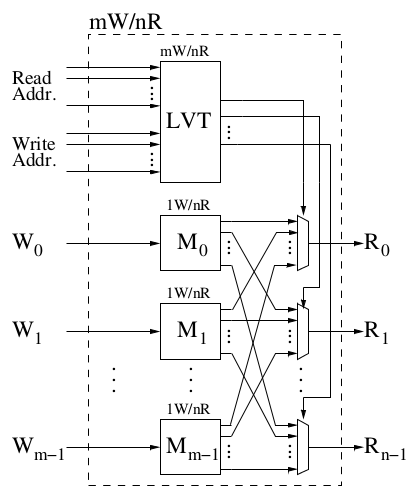
\includegraphics[width=2.0in]{lvt}
\caption{A generalized mW/nR memory implemented using a Live Value Table}
\label{lvt}
\end{figure}

The LVT allows a banked design to behave like a true multi-ported design by directing reads to appropriate banks based on which bank holds the most recent or “live” write value. Each write updates its own replicated memory bank (M) and updates its entry at the same address in the LVT. For each read, the LVT selects the memory bank that holds the most recently written value for the requested memory address \cite{LaForest}.

We propose an asynchronous controller in order to minimize the delay between thread request and memory response. We focus our analysis on the Minimum Input Arrival Time Before Clock (MIATBC) and the Maximum Output Required Time After Clock (MORTAC) variables for studying the combinational circuit delay and the routing delay in the FPGA.



\vspace{7pt}
\section{Implementation}
We have based our designs and tests in the Atlys Spartan-6 FPGA development board from Digilent. This low class development board has been sufficient to test the multi-ported memories with a Microblaze embedded microprocessor.

Due to the limits in the availability of BRAMs in FPGAs, and as we try to create shared memories of high capacity as those available in current GPGPUs, we have decided to use an architecture that minimizes the use of BRAMs. That means, for an N-ported shared memory, we will be using N/2 BRAMs, taking advantage of the two independent ports already available in all the BRAMs.

According to this architecture, an N-ported shared memory has, in fact, N ports available, but only 2 ports can access the same BRAM. In order to make all the memory address space available to all threads, we have used a multiplexer in each BRAM port. We have calculated the combinational equation \eqref{1} of the control signals for the input multiplexers. In which N is the number of ports, n are the multiplexer control signals and K(w) is the logic function that determines whether the kernel w is requesting access to the multiplexer’s BRAM port. This equation can be used for any $N=2^m$ number of ports, being m a positive integer.

\begin{multline} \label{1}
  A(n) = \neg \sum_{a=0}^{N/2^{n+1}-1}
         \sum_{b=0}^{N/2^{log(N)-n}-1} K(2^{n+1}a+b) \\
         \prod_{c=0}^{a-1}
         \prod_{d=0}^{N/2^{log(N)-n}-1} \neg K(2^{n+1}c+2b-d-1)
\end{multline}

The controller for the memory output has also been implemented with multiplexers, but in this case, with a trivial equation \cite{Source}.

Although this method allows all threads to access any address in the memory address space, collisions may occur when more than two threads want to have access to memory addresses that are in the same BRAM, as BRAMs can only serve up to two independent requests due to their true dual port configuration.

As our configuration is set to minimize the use of BRAMs and, therefore, we can not use replication methods, the only way to serve all the request is to serialize them. Due to the philosophy of parallel computation, normally different threads are supposed to only access different memory address space tiles at the same time and, because of synchronization methods, they may want to access at the same time the same memory address. That is why we have also tested a broadcast feature in the implementation. When various or all the threads request access to the same memory address, the BRAM can output the same data to these threads without needing to serialize the requests.

Writing VHDL code for creating these memories is a really complex task, especially when trying to implement the combinational equation of the control signals for the multiplexers. That is why, instead, we have created a program in C that automatically generates the VHDL code for the memories. Although a little bit slower at the beginning, programming the C code, it has helped a lot creating big shared memories (i.e.: a 64 ports shared memory VHDL code resulted in more than 75000 lines of code and 8000000 characters in the file). Furthermore, we have automated the process of synthesis report and graphics generation with the aid of Tcl and Bash script languages. All the code has been published under the General Public Licence (GPL) \cite{Source}.



\vspace{7pt}
\section{Results}

In all of the graphics, the x axis always represents the number of ports in the shared memory while the y axis usually represents the delay in nanoseconds (exception: in the SLICE\_LUTS graphic, it represents the number of LUTs used).

The BRAM utilization increases, of course, linearly with the number of ports with a $1/2$ ratio. For both the broadcast and no-broadcast implementations, the LUT utilization increases exponentially (Fig. \ref{luts}), which is something expected due to the increasing complexity of the logic equation. We can also notice that adding the broadcast feature does not add a lot of complexity to the logic equation and, therefore, to the combinational circuit.

\begin{figure}[h]
\centering
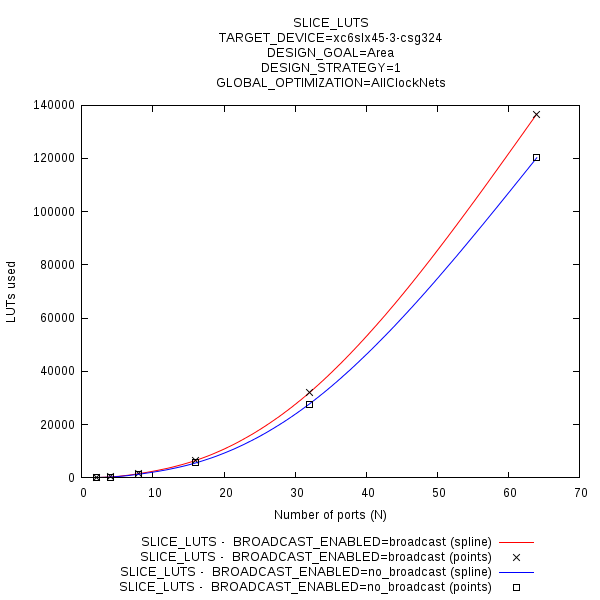
\includegraphics[width=3.5in]{luts}
\caption{Slice LUTs utilization}
\label{luts}
\end{figure}

Although this could be a good indicator for starting to think that the broadcast feature may be worth implementing, comparing MIATBC and MORTAC delays in nanoseconds for both implementations, we discover that, in fact, adding this feature results in too high delays and low operating frequencies for the memories (Fig. \ref{miatbc_vs_mortac}).

\begin{figure}[h]
\centering
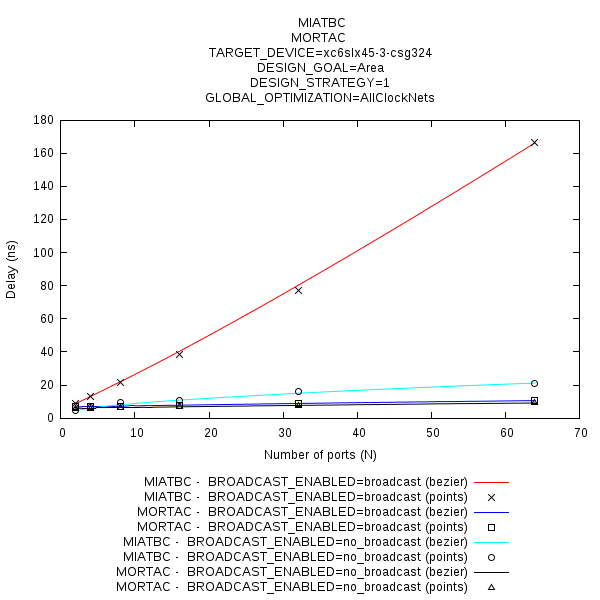
\includegraphics[width=3.5in]{miatbc_vs_mortac}
\caption{MIATBC and MORTAC delays comparison for both broadcast and no-broadcast implementations}
\label{miatbc_vs_mortac}
\end{figure}

As the LUT utilization is not so different, we should try to guess now why does this huge difference exist in the MIATBC. Dividing the MIATBC delays into those produced by the combinational circuit and those produced by the routing in the FPGA, we get the answer (Fig. \ref{miatbc_logic_vs_route}). Although the circuit is not much more complex, the fact that the synthesizer has to create more connections between elements adds a huge delay due to routing wires in the FPGA.

\begin{figure}[h]
\centering
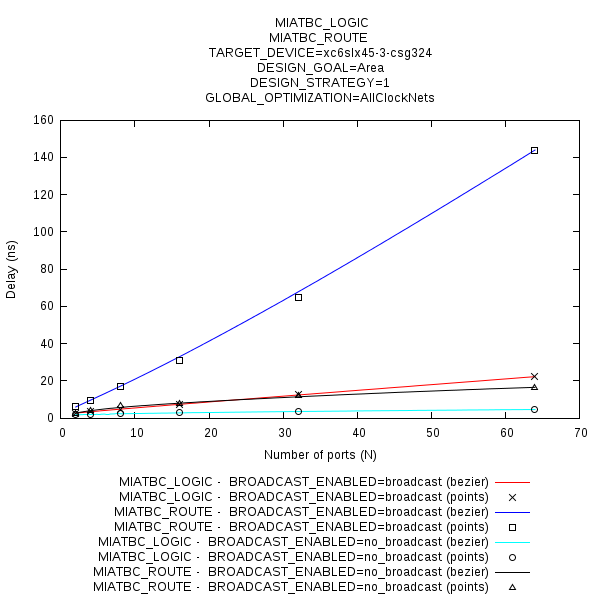
\includegraphics[width=3.5in]{miatbc_logic_vs_route}
\caption{MIATBC delays produced by the combinational circuit and the routing}
\label{miatbc_logic_vs_route}
\end{figure}

This huge difference in the MIATBC delay is enough to discard the possibility of creating broadcast enabled memories, even if we see that the MORTAC delay difference is small between both implementations. The gain obtained when we hit a multiple request to the same address case is much smaller than the loss produced by the constant delay in the input of the memory controller.

\begin{figure}[h]
\centering
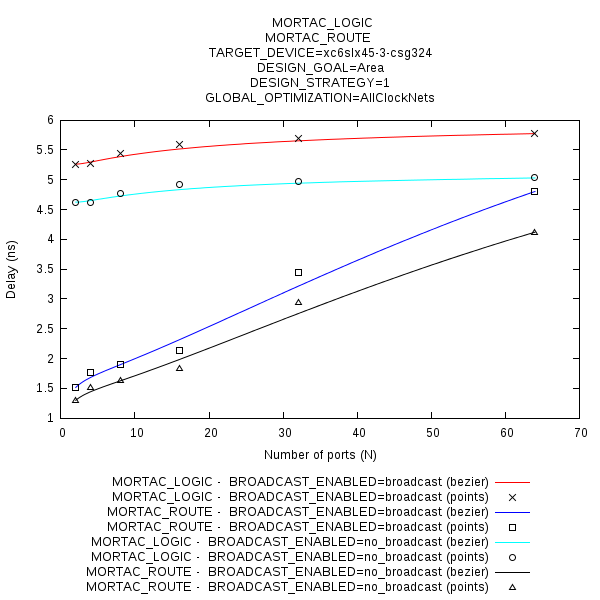
\includegraphics[width=3.5in]{mortac_logic_vs_route}
\caption{MORTAC delays produced by the combinational circuit and the routing}
\label{mortac_logic_vs_route}
\end{figure}

As we can observe in the graphics (Fig. \ref{miatbc_vs_mortac_no_broadcast}), even for the no broadcast architecture, the highest delay is caused by the MIATBC and, especially (Fig. \ref{miatbc_delays_no_broadcast}), by the routing delay at the input.

\begin{figure}[h]
\centering
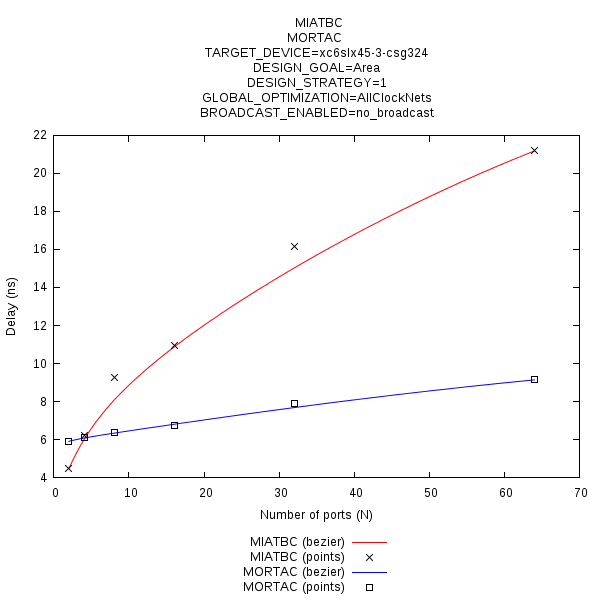
\includegraphics[width=3.5in]{miatbc_vs_mortac_no_broadcast}
\caption{MORTAC and MIATBC delays for the no-broadcast architecture}
\label{miatbc_vs_mortac_no_broadcast}
\end{figure}

\begin{figure}[h]
\centering
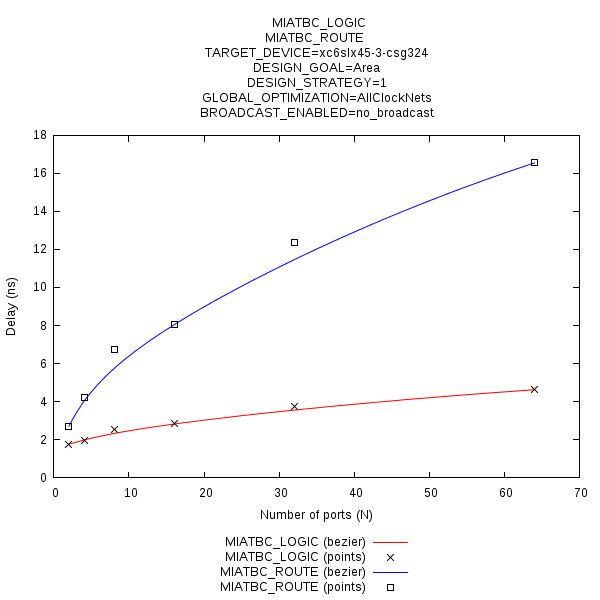
\includegraphics[width=3.5in]{miatbc_delays_no_broadcast}
\caption{MIATBC delays produced by the combinational circuit and the routing for the no-broadcast architecture}
\label{miatbc_delays_no_broadcast}
\end{figure}

The maximum path delay is the sum of the MORTAC and MIATBC delays, resulting in a value between 16 and 40 nanoseconds, depending on the number of ports of the memory. That means the maximum operating frequency is between 62.5 and 25 MHz, depending on the number of ports (between 2 and 64 ports).

We can also notice in the graphics that the delays do not always fit well in the bezier curve. In fact, we can notice how, generally, the derivative of a better fitted curve would decrease until reaching 16 ports and then would increase with higher derivative again. That is because, in fact, in the FPGA we can find 16 ports multiplexers and, therefore, we are maximizing their utilization when we set the number of ports to 16. For lower value of ports the utilization of this multiplexers is not optimal, and for higher, the synthesizer has to use various multiplexers to create a $>16$ ports multiplexer.



\vspace{7pt}
\section{Conclusion}
FPGA systems provide efficient BRAMs, but with only two ports. Although conventional approaches may be faster and although we can find even more efficient approaches as proposed by Charles Eric LaForest (LVT-based memories), we introduced a new architecture that provides true multiported shared memories while minimizing the use of BRAMs to generate the address space.

Our memories do not use replication methods, maximizing the utilization of each BRAM. On the other hand, they are slow compared to other approaches and tend to use more area in the FPGA.

We have to remark that: (i) our architecture is by no means effective when adding the broadcast feature; (ii) our architecture behaves as a real N-ported shared memory only when all threads access different memory address space tiles, otherwise the memory accesses are serialized\footnote{The serialization of requests occurs only when more than two threads want to access simultaneously a single BRAM (two consecutive memory address space tiles).}.

In summary, an asynchronous shared memory controller that does not make use of replication methods could be well implemented in an ASIC, but would hardly outperform other approaches when implemented in an FPGA, which has limited flexibility for creating the combinational circuit and making the routing.

We expect that our architecture may be improved when combined with other methods. Just as the LVT makes use of replication and has better performance when combined with multi-pumping methods.



\vspace{7pt}
\begin{thebibliography}{1}

\bibitem{Source}
Source code,
\emph{https://github.com/Peque/fastcuda/archive/0.1.tar.gz}

\bibitem{LaForest}
C. E. LaForest and J. G. Steffan,
\emph{Efficient Multi-Ported Memories for FPGAs},
In Proceedings of the 18th annual ACM/SIGDA international symposium on Field
Programmable Gate Arrays, FPGA ’10, New York, NY, USA, 2010. ACM.

\bibitem{LaForestXOR}
C. E. LaForest, M. G. Liu, E. R. Rapati, and J. G. Steffan,
\emph{Multi-Ported Memories for FPGAs via XOR},
In Proceedings of the 20th annual ACM/SIGDA international symposium on Field
Programmable Gate Arrays, FPGA '12, New York, NY, USA, 2012. ACM.

\bibitem{ProgrammingMassivelyParallelProcessors}
D. B. Kirk and W. W. Hwu,
\emph{Programming Massively Parallel Processors},
Morgan Kaufmann, 2010.

\bibitem{XilinxBRAM}
Xilinx,
\emph{IP Processor Block RAM specification},
2011.

\bibitem{XilinxSPARTAN6}
Xilinx,
\emph{Spartan-6 FPGA Configurable Logic Block User Guide},
2010.

\bibitem{XilinxSynthesis&Simulation}
Xilinx,
\emph{Synthesis and Simulation Design Guide},
2012.

\bibitem{XilinxSPARTAN6BRAM}
Xilinx,
\emph{Spartan-6 FPGA Block RAM Resources User Guide},
2011.

\bibitem{XilinxSPARTAN6lib}
Xilinx,
\emph{Spartan-6 Libraries Guide for HDL Designs},
2012.

\bibitem{XilinxuBlaze}
Xilinx,
\emph{MicroBlaze Processor Reference Guide},
2012.

\bibitem{XilinxuEDK}
Xilinx,
\emph{Embedded System Tools Reference Manual},
2012.

\end{thebibliography}



\end{document}
